\documentclass[11pt,a4paper,oldfontcommands,oneside]{memoir}
\usepackage[utf8]{inputenc}
\usepackage{microtype}
\usepackage[dvips]{graphicx}
\usepackage{xcolor}
\usepackage{times}
\usepackage{graphicx}
\usepackage{amsmath}
\usepackage[spanish]{babel}
\usepackage[
breaklinks=true,colorlinks=true,
%linkcolor=blue,urlcolor=blue,citecolor=blue,% PDF VIEW
linkcolor=black,urlcolor=black,citecolor=black,% PRINT
bookmarks=true,bookmarksopenlevel=2]{hyperref}

\usepackage{geometry}
% PDF VIEW
% \geometry{total={210mm,297mm},
% left=25mm,right=25mm,%
% bindingoffset=0mm, top=25mm,bottom=25mm}
% PRINT
\geometry{total={210mm,297mm},
left=20mm,right=20mm,
bindingoffset=10mm, top=25mm,bottom=25mm}

\OnehalfSpacing
%\linespread{1.3}

%%% CHAPTER'S STYLE
\chapterstyle{bianchi}
%\chapterstyle{ger}
%\chapterstyle{madsen}
%\chapterstyle{ell}
%%% STYLE OF SECTIONS, SUBSECTIONS, AND SUBSUBSECTIONS
\setsecheadstyle{\Large\bfseries\sffamily\raggedright}
\setsubsecheadstyle{\large\bfseries\sffamily\raggedright}
\setsubsubsecheadstyle{\bfseries\sffamily\raggedright}


%%% STYLE OF PAGES NUMBERING
%\pagestyle{companion}\nouppercaseheads 
%\pagestyle{headings}
%\pagestyle{Ruled}
\pagestyle{plain}
\makepagestyle{plain}
\makeevenfoot{plain}{\thepage}{}{}
\makeoddfoot{plain}{}{}{\thepage}
\makeevenhead{plain}{}{}{}
\makeoddhead{plain}{}{}{}


\maxsecnumdepth{subsection} % chapters, sections, and subsections are numbered
\maxtocdepth{subsection} % chapters, sections, and subsections are in the Table of Contents


%%%---%%%---%%%---%%%---%%%---%%%---%%%---%%%---%%%---%%%---%%%---%%%---%%%

\begin{document}

%%%---%%%---%%%---%%%---%%%---%%%---%%%---%%%---%%%---%%%---%%%---%%%---%%%
%   TITLEPAGE
%
%   due to variety of titlepage schemes it is probably better to make titlepage manually
%
%%%---%%%---%%%---%%%---%%%---%%%---%%%---%%%---%%%---%%%---%%%---%%%---%%%
\thispagestyle{empty}

{%%%
\sffamily
\centering
\Large

~\vspace{\fill}

\includegraphics[scale=.85]{logo1.png} \\
{\huge 
\vspace{4cm}
Simulación de Cinemática Directa e Inversa de Manipuladores Seriales
}
\vspace{2.5cm}

{\LARGE
César Omar Alvarado Contreras\\
Jonathan Fonseca Camarena\\
Marcos Manzo Torres\\
Eduardo Robles Vázquez\\
Víctor Gabriel Tapia Casillas
}

\vspace{3.5cm}

Universidad Politécnica de la Zona Metropolitana de Guadalajara

\vspace{2.5cm}

Profesor: Carlos Enrique Morán Garabito

\vspace{\fill}

27 de septiembre del 2019

%%%
}%%%

\vspace{.5cm}
\hfill\break




\tableofcontents*

\clearpage

%%%---%%%---%%%---%%%---%%%---%%%---%%%---%%%---%%%---%%%---%%%---%%%---%%%
%%%---%%%---%%%---%%%---%%%---%%%---%%%---%%%---%%%---%%%---%%%---%%%---%%%

\chapter{Introducción}
\section{Objetivo}
Demostrar las características cinemáticas directas de nuestro prototipo de robot mediante cálculos y simulaciones en un software de diseño.
\section{Investigación Previa}
\textbf{Convención Denavit-Hartenberg}. \\\
Jacques Denavit y Richard Hartenberg introdujeron esta convención en 1955 con el fin de estandarizar los marcos de coordenadas para los enlaces espaciales.
Richard Paul demostró su valor para el análisis cinemático de los sistemas robóticos en 1981. Si bien se han desarrollado muchas convenciones para adjuntar marcos de referencia, la convención Denavit-Hartenberg sigue siendo un enfoque popular. \\
Se trata de un procedimieto sistemático para describir la estructura cinemática de una cadena articulada constituida por articulaciones con. un solo grado de libertad. \\ Para ello, a cada articulación se le asigna un Sistema de Referencia Local con origen en un punto Qi y ejes ortonormales [Xi, Yi, Zi], comenzando con un primer S.R fijo e inmóvil dado por los ejes [x0, Y0, Z0], anclado a un punto fijo Q0 de la Base sobre la que está montada toda la estructura de la cadena.\\ Este Sistema de Referencia no tiene por qué ser el Universal con origen en (0,0,0) y la Base canónica
\section{Materiales}
-Computadora con software (SolidWorks) 
\chapter{Desarrollo}
El ánalisis de la Cinemática Directa será hecho a traves de la convención de Denavit-Hartenberg.\\
Primero hacemos el ánalisis de los ejes de nuestro robot.\\
\begin{center}
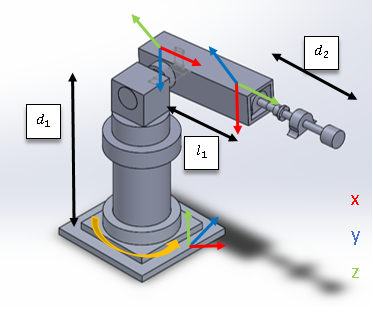
\includegraphics[scale=.65]{brazo.png} \\
\end{center}

Con base al ánalisis anterior procedemos a hacer la tabla DH. \\
\begin{center}
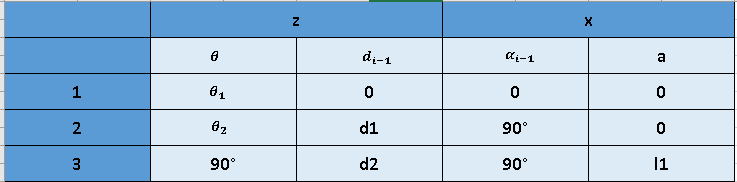
\includegraphics[scale=.65]{table.png} \\
\end{center}

Una vez realizada la tabla DH podemos hacer las matrices: \\

\[^{i-1}A_{i}= 
\begin{bmatrix}
    Cos(\theta_{i})       & -Cos(\alpha_{i})Sin(\theta_{i}) & Sin(\alpha_{i})Sin(\theta_{i}) & a_{i}Cos(\theta_{i}) \\
    
    Sin(\theta_{i})       & Cos(\alpha_{i})Cos(\theta_{i}) & -Sin(\alpha_{i})Cos(\theta)  & a_{i}Sin(\theta_{i}) \\
    
    0       & Sin(\alpha_{i}) & Cos(\alpha_{i}) & a_{i} \\
    
    0       & 0 & 0  & 1
\end{bmatrix}
\]

Basándose en la tabla, sustituímos los valores, la primera matriz empieza con los valores de la primera fila de la tabla DH y se continúa con ese orden respectivamente, hasta que se obtengan las matrices con el siguiente lineamiento: \\
\[^{0}A_{1}= 
\begin{bmatrix}
    Cos(\theta)       & -Cos(0)Sin(\theta) & Sin(0)Sin(\theta) & 0Cos(\theta) \\
    
    Sin(\theta)       & Cos(0)Cos(\theta) & -Sin(0)Cos(\theta)  & 0Sin(\theta) \\
    
    0       & Sin(0) & Cos(0) & 0 \\
    
    0       & 0 & 0  & 1
\end{bmatrix}
\]

\[^{1}A_{2}= 
\begin{bmatrix}
    Cos(\theta)       & -Cos(90)Sin(\theta) & Sin(90)Sin(\theta) & 0Cos(\theta) \\
    
    Sin(\theta)       & Cos(90)Cos(\theta) & -Sin(90)Cos(\theta)  & 0Sin(\theta) \\
    
    0       & Sin(90) & Cos(90) & d_{i} \\
    
    0       & 0 & 0  & 1
\end{bmatrix}
\]

\[^{2}A_{3}= 
\begin{bmatrix}
    Cos(90)       & -Cos(90)Sin(90) & Sin(90)Sin(90) & l_{1}Cos(90) \\
    
    Sin(90)       & Cos(90)Cos(90) & -Sin(90)Cos(90)  & l_{1}Sin(90) \\
    
    0       & Sin(90) & Cos(90) & d_{2} \\
    
    0       & 0 & 0  & 1
\end{bmatrix}
\] \\

Simplificando las matrices anteriores, éstas quedarán de la siguiente manera:\\

\[^{0}A_{1}= 
\begin{bmatrix}
    Cos(\theta)       & -Sin(\theta) & 0 & 0 \\
    
    Sin(\theta)       & Cos(\theta) & 0  & 0 \\
    
    0       & 0 & 1 & 0 \\
    
    0       & 0 & 0  & 1
\end{bmatrix}
\]

\[^{1}A_{2}= 
\begin{bmatrix}
    Cos(\theta)       & 0 & Sin(\theta) & 0 \\
    
    Sin(\theta)       & 0 & -Cos(\theta)  & 0 \\
    
    0       & 1 & 0 & d_{i} \\
    
    0       & 0 & 0  & 1
\end{bmatrix}
\]

\[^{2}A_{3}= 
\begin{bmatrix}
    0       & 0 & 1 & 0 \\
    
    1       & 0 & 0  & l_{1} \\
    
    0       & 1 & 0 & d_{2} \\
    
    0       & 0 & 0  & 1
\end{bmatrix}
\] \\
Una vez obtenidas las matrices, pasamos a multiplicarlas: \\
\[A_{r}= ^{0}A_{1}*^{1}A_{2}*^{2}A_{3}
\]
Dando así la siguiente matriz: \\
\[A_{r}= 
\begin{bmatrix}
    0 & 1 & Cos^{2}(\theta)-Sin^{2}(\theta) & 2d_{2}Sin(\theta)Cos(\theta) \\
    
    0 & Sin^{2}(\theta)-Cos^{2}(\theta) & 2Sin(\theta)Cos(\theta)  & l_{1}+d_(1) \\
    
    1 & 0 & 0 & l_{1}+d_{1} \\
    
    0 & 0 & 0  & 1
\end{bmatrix}
\]


\chapter{Conclusión}
\section{Alvarado Contreras César Omar}
Al poner los ejes correspondientes de la base del robot es algo entretenido a la hora de no saber que rotación debe proponerse para el tipo de máquina que se está mapeando en las articulaciones de nuestro robot compuesto, a la hora de hacer la matriz se siguió un ejemplo en un libro “La representación Denavit-Hartenberg” en el cual se explica como se desarrolla en mi caso me guie para hacer la multiplicaciones correspondientes de las matrices 
\section{Fonseca Camarena Jonathan}
En resumen, los futuros robots tendrían muchos de los atributos de los seres humanos. La robótica es una tecnología que solo puede destinarse al beneficio de la humanidad. Sin embargo, como otras tecnologías, se necesita de personas que los manejen hoy aun, como en esta práctica, aprendimos que tienen un universo, dirección y perspectiva, el espacio es algo que tenemos en común los robots con los humanos, por eso, aprendimos lo importantes de las referencias y como aplicarlas a la tabla DH y sus pasos, después como la traducimos a matrices que son las que determinara el movimiento del Robot, insisto, la investigación fue fundamental para hacer esta práctica
\section{Manzo Torres Marcos}
l realizar la cinematica y desplazamientos de un robot, todas las cosas se unen para llegar al productor final y al correcto funcionamiento. Se debe tener en cuenta que cada configuración de robot nos aroja un distinto panorama de trabajo, por lo que para facilitar las operaciones resulta más sencillo definir desde un principio las características específicas y lo que queremos hacer con ello. Es la primera vez abordamos este tema, aunque resultó un poco difícil fue de gran satisfacción llegar a un resultado concreto y que nos ayuda a avanzar en nuestro proyecto cuatrimestral
\section{Robles Vázquez Eduardo}
Con esta práctica aprendimos a aplicar los pasos de la convención de Denavit-Hartenberg a un proyecto real, que es la parametrización de nuestro brazo robot, todo esto con el fin de tener una perspectiva de la ubicación y dirección del robot y por ende poder controlarlo. No es dificil, solo un poco laborioso todo este proceso.
\section{Tapia Casillas Víctor Gabriel}
Con esta práctica pudimos sacar los parámetros de los ejes y los distintos movimientos capaces de realizar nuestro robot, lo cual nos será de mucha ayuda al momento que empecemos a programar los movimientos de nuestro robot en ROS.


\vspace{2cm}
\hfill
\cite{Nobody06}
\bibliographystyle{unsrt}
\bibliography{prueba}
\end{document}

}